\part{Python programming I}
\section{Introduction}
\subsection*{General}
\begin{frame}[label=contents_prog1]
  \frametitle{Today's outline}
  \mode<beamer>{
    \only<1>{\tableofcontents}
  }
  \only<2>{\tableofcontents[currentsection]}
\end{frame}

\begin{frame}
 \frametitle{Why should you learn something about programming?}
 \begin{itemize}[<+->]
  \item Scientific techniques depend in an increasing fashion upon computer programs and simulation methods
  \item Knowledge of programming allows you to automate routine tasks 
  \item Ability to understand algorithms by inspection of the code 
  \item Learn to think by dissecting a problem into smaller bits 
 \end{itemize}\vskip2em
 \begin{columns}
  \column<1->{0.23\textwidth}
  \tikz\node[circle,draw,very thick,maincolor,
           text=white,minimum size=\columnwidth,
           path picture={
               \node at (path picture bounding box.center){
                   \includegraphics[width=\columnwidth]{sim1.png}
               };
           }]{};
  \column<2->{0.23\textwidth}
  \tikz\node[circle,draw,very thick,maincolor,
           text=white,minimum size=\columnwidth,
           path picture={
               \node at (path picture bounding box.center){
                   \includegraphics[width=1.1\columnwidth]{automate.jpg}
               };
           }]{};
  \column<3->{0.23\textwidth}
  \tikz\node[circle,draw,very thick,maincolor,
           text=white,minimum size=\columnwidth,
           path picture={
               \node at (path picture bounding box.center){
                   \includegraphics[width=1.2\columnwidth]{algorithm.jpg}
               };
           }]{};
  \column<4>{0.23\textwidth}
  \tikz\node[circle,draw,very thick,maincolor,
           text=white,minimum size=\columnwidth,
           path picture={
               \node at (path picture bounding box.center){
                   \includegraphics[width=1.5\columnwidth]{dissect.jpg}
               };
           }]{};
 \end{columns}
\end{frame}

\begin{frame}
 \frametitle{Introduction to programming}
 \begin{block}{What is a program?}
  \emph{A program is a sequence of instructions that is written to perform a certain task on a computer.} % SOURCE http://www.greenteapress.com/thinkpython/html/thinkpython002.html
  \end{block}
  \begin{itemize}
    \item The computation might be something mathematical, a symbolic operation, image analysis, etc.%such as solving a system of equations or finding the roots of a polynomial
    % \item It can also be a symbolic computation, such as searching and replacing text in a document 
    % \item A program may even be used to compile another program
    % \item A program consists of one or more \emph{algorithms}
  \end{itemize}
  \begin{block}{Program layout}
    \begin{enumerate}
        \item Input (Get the radius of a circle)
        \item Operations (Compute and store the area of the circle)
        \item Output (Print the area to the screen)
    \end{enumerate}
  \end{block}
\end{frame}

\begin{frame}
\frametitle{Versatility of Python}
\centering\includegraphics[width=0.9\textwidth]{python_versatility.pdf}
\end{frame}

\begin{frame}
\frametitle{Versatility of Python: ODE solver}
\includegraphics[width=\textwidth]{odesol.png}
\end{frame}

\begin{frame}[fragile]
\frametitle{Versatility of Python: Image analysis}
\begin{columns}
  \column{0.5\textwidth}
\begin{lstlisting}
# Importing necessary lirbraries
import numpy as np
from scipy import ndimage
from PIL.Image import fromarray
from skimage import io, color, feature, measure

# Loading and processing image 
I = io.imread('bub0.png')
BW = color.rgb2gray(I)
E = feature.canny(BW) 
F = ndimage.binary_fill_holes(E)
\end{lstlisting}  
\column{0.5\textwidth}
  \vfill
  \includegraphics<1>[width=\columnwidth]{bub1.png}
  \includegraphics<2>[width=\columnwidth]{bub2.png}
  \includegraphics<3>[width=\columnwidth]{bub3.png}
  \includegraphics<4>[width=\columnwidth]{bub4.png}
\end{columns}
\end{frame}

\begin{frame}
\frametitle{Versatility of Python: Curve fitting}
\centering\includegraphics[width=\textwidth]{cftool.png}
\end{frame}

\begin{frame}[fragile]
  \frametitle{Getting started}
   Start Python, and enter the following commands on the command line. Evaluate the output.
   \pause
   \begin{lstlisting}[language=Python,numbers=none]
>> 2 + 3        # Some simple calculations
>> 2 * 3
>> 2 * 3**2     # Powers are done using ** (*@ \pause @*)
>> a = 2        # Storing values into the workspace
>> b = 3
>> c = (2 * 3)**2  # Parentheses set priority
>> 8 / a - b (*@ \pause @*)
>> import math  # Mathematical functions can be used 
>> math.sin(a)  
>> math.sin(0.5 * math.pi)  # math.pi is an internal Python variable
>> import cmath  # for working with complex numbers
>> cmath.sqrt(-1)  # ... as are imaginary numbers    
   \end{lstlisting}
 \end{frame}
 

 %% PRINTING
 \begin{frame}[fragile]
  \frametitle{Printing and formatting results}
  In Python, you can control the display format of the output of a command using various formatting methods such as `str.format()`, f-strings, or by using formatting specifiers while printing with `print()`. These methods only involve changing the way the numbers are displayed, not the underlying representation.
  
  \begin{lstlisting}[language=Python,numbers=none]
>> # Using str.format()
>> a = 19/4
>> print("{:.2f}".format(a)) # 2 decimal places
>> b = a**(-6)
>> print("{:.10f}".format(b)) # 10 decimal places
>> 
>> # Using f-strings (Python 3.6+)
>> c = (21)**0.5
>> print(f"{c:.10f}") # 10 decimal places
>> d = (2.71828)**(-c) 
>> print(f"{d:.2e}") # Scientific notation with 2 decimal places
>> 
>> # Using print formatting
>> print("{:.2f}".format(d)) # 2 decimal places
  \end{lstlisting}
\end{frame}

 
 {\nologo
 \begin{frame}[fragile]
  \frametitle{A few helpful things}
  \begin{itemize}[<+->]
    \item Using the \keystroke{$\uparrow$} and \keystroke{$\downarrow$} keys, you can cycle through recent commands
    \item Typing part of a command and pressing \keystroke{Tab} completes the command and lists the possibilities
    \item If a computation takes too long, you can press \keystroke{Ctrl}+\keystroke{C} to stop the program and return to the command line. Note that you may end up with incomplete results in the workspace.
    \item Sequences of commands (programs, scripts) are contained as py-files, plain text files with the \lstinline$.py$ extension.
    \item Python scripts can also be contained in jupyter notebooks, which have extension \lstinline$.ipynb$.
    \item Such py-files must be in the \emph{current working directory} or in the Python \emph{path}, the locations where Python searches for a command. If you try to run a script that is not in the path, Python will throw an Exception/Error.
    \item Anything following a \lstinline$#$ symbol is regarded as a comment
    \item There are several keyboard shortcuts (vary with text editor) that will make coding much more efficient.
  \end{itemize}
\end{frame}
}

\begin{frame}[fragile]
\frametitle{Python help, documentation, resources}
\begin{itemize}[<+->]
  \item Refer to the Python documentation at \href{https://docs.python.org/3/}{Official documentation}.
  \begin{itemize}
    \item Try for instance: \lstinline$help(print)$ or \lstinline$help(help)$.
  \end{itemize}
  \item We supplied a number of basic Canvas modules: Python Crash Course, including small exercises.
  \item Python Crash Course, 2nd Edition by Eric Matthes.
  \item Search the web, Reddit, YouTube, etc.
\end{itemize}
\end{frame}

\section{Data structures}
\subsection*{Introduction}
\againframe<2>{contents_prog1}
\begin{frame}
 \frametitle{Terminology}
 \begin{description}
  \item[Variable] Piece of data stored in the computer memory, to be referenced and/or manipulated
  \item[Function] Piece of code that performs a certain operation/sequence of operations on given input
  \item[Operators] Mathematical operators (e.g. \lstinline$ + - *$ or \lstinline$/$), relational (e.g. \lstinline$< >$or \lstinline$==$, and logical operators (\lstinline$and$, \lstinline$or$)
  \item[Script] Piece of code that performs a certain sequence of operations without specified input/output
  \item[Expression] A command that combines variables, functions, operators and/or values to produce a result.
 \end{description}
\end{frame}

\begin{frame}[fragile]
 \frametitle{Variables in Python}
  \begin{itemize}
   \item Python stores variables in the \emph{namespace}\pause
   \item You should recognize the difference between the \emph{identifier} of a variable (its name, e.g. \lstinline$x$, \lstinline$setpoint_p$), and the data that it actually stores (e.g. 0.5)\pause
   \item Python also defines a number of functions by default, e.g. \lstinline$min$, \lstinline$max$ or \lstinline$sum$.\pause
   \item You can assign a variable by the \lstinline$=$ sign:
   \begin{lstlisting}[language=Python, numbers=none]
>> x = 4*3
>> x
12
   \end{lstlisting}\pause
   \item If you don't assign a variable, it will be stored in \lstinline$_$
   \item In most text editors, all variables are cleared automatically before the next execution. 
 \end{itemize}
\end{frame}

\begin{frame}[fragile]
  \frametitle{Datatypes and variables}
  Python uses different types of variables:
      \begin{longtable}{l!{\vrule}l}
       Datatype        & Example \\ \hline
       \lstinline$str$    & \lstinline$'Wednesday'$ \\
       \lstinline$int$    & \lstinline$15$ \\
       \lstinline$float$  & \lstinline$0.15$ \\
       \lstinline$list$   & \lstinline$[0.0, 0.1, 0.2]$ \\
       \lstinline$dict$   & \lstinline${'name': 'word', "n": 2}$ \\
       \lstinline$bool$   & \lstinline$False$ \\
       \lstinline$tuple$  & \lstinline$(True, False)$ \\
     \end{longtable}
 \end{frame}


 %% LISTS SECTION
 \subsection*{Lists}
 \begin{frame}[fragile]
   \frametitle{Lists in Python (1)}
   A list:
   \begin{lstlisting}[language=Python,numbers=none]
>> v = [0, 1, 2, 3]
   \end{lstlisting}\pause
   Access (i.e., read) an entry in a list:
   \begin{lstlisting}[language=Python,numbers=none]
>> v[1]
 1
   \end{lstlisting}\pause
   Manipulate the value of that entry:
   \begin{lstlisting}[language=Python,numbers=none]
>> v[1] = 47
   \end{lstlisting}\pause
   Get a slice of a list:
   \begin{lstlisting}[language=Python,numbers=none]
>> v[1:4] # This will give the elements from index 1 to index 3
 [47, 2, 3]
   \end{lstlisting}\pause
   Extending a list with another list:
   \begin{lstlisting}[language=Python,numbers=none]
>> w = v + [4, 5, 6]
>> w
 [0, 47, 2, 3, 4, 5, 6]
   \end{lstlisting}
 \end{frame}
 
 \begin{frame}[fragile]
   \frametitle{Lists in Python (2)}
   Create a list with a range of numbers:
   \begin{lstlisting}[language=Python,numbers=none]
>> a = list(range(1, 11))     # Creates a list from 1 to 10
   \end{lstlisting}\pause
   List comprehensions can be used to create lists with more complex patterns:
   \begin{lstlisting}[language=Python,numbers=none]
>> x = [i/10 for i in range(-10, 11)]   # Creates a list from -1 to 1 with a step of 0.1
   \end{lstlisting}\pause
   Manipulating multiple components using slicing and a loop:
   \begin{lstlisting}[language=Python,numbers=none]
>> y = list(range(11))  # Creates a list from 0 to 10
>> for i in [0, 3, 4, 5, 6]: 
>>     y[i] = 1
   \end{lstlisting}\pause
   Or (by supplying a list instead of a scalar):
   \begin{lstlisting}[language=Python,numbers=none]
>> y[0:2] = [16, 19]  # Sets y[0] to 16 and y[1] to 19
   \end{lstlisting}
 \end{frame}
 

\begin{frame}[fragile]
 \frametitle{Practice}
 Given a vector 
 \[ 
    x = \left[2 \ 4 \ 6 \ 8 \ 10 \ 12 \ 14 \ 16 \ 18 \ 20 \ 30 \ 40 \ 50 \ 60 \ 70 \ 80 \right]
 \]
 \begin{itemize}
  \item Find a way to define the vector without typing all individual elements\pause
  \item Investigate the meaning of the following commands:
  \begin{lstlisting}[language=Python, numbers=none]
>> x[2]            
>> x[0:5]          
>> x[:-1]          
>> y = x[4:]       
>> y[3]            
>> y.pop(3)      
>> sum(x)    
>> max(x)       
>> min(x) 
>> x[::-1]       
    \end{lstlisting}    
 \end{itemize}
\end{frame}

%% STRING SECTION
\subsection*{Strings}
\begin{frame}[fragile]
  \frametitle{Strings in Python (1)}
  Creating a string:
  \begin{lstlisting}[language=Python,numbers=none]
>> s = "Hello, world!"
  \end{lstlisting}\pause
  Accessing a character in a string:
  \begin{lstlisting}[language=Python,numbers=none]
>> s[7]
'w'
  \end{lstlisting}\pause
  Getting a substring:
  \begin{lstlisting}[language=Python,numbers=none]
>> s[7:12]
'world'
  \end{lstlisting}\pause
  Finding the length of a string:
  \begin{lstlisting}[language=Python,numbers=none]
>> len(s)
13
  \end{lstlisting}
\end{frame}

%% TUPLES SECTION
\subsection*{Tuples}
\begin{frame}[fragile]
  \frametitle{Tuples in Python}
  Creating a tuple:
  \begin{lstlisting}[language=Python,numbers=none]
>> t = (1, 2, 3)
  \end{lstlisting}\pause
  Accessing an element of a tuple:
  \begin{lstlisting}[language=Python,numbers=none]
>> t[1]
2
  \end{lstlisting}\pause
  Tuples are immutable, so we can't change their elements. However, we can create a new tuple based on the old one:
  \begin{lstlisting}[language=Python,numbers=none]
>> t = t + (4, )
  \end{lstlisting}\pause
  Finding the length of a tuple:
  \begin{lstlisting}[language=Python,numbers=none]
>> len(t)
4
  \end{lstlisting}
\end{frame}

\begin{frame}[fragile]
  \frametitle{Practice}
  Given a tuple
  \[
     t = (1, 2, 3, 4, 5, 6)
  \]
  \begin{itemize}
   \item Access and print the third element of the tuple.\pause
   \item Try to change the value of the second element of the tuple.\pause
   \item Create a new tuple by concatenating a second tuple \((7, 8, 9)\) to the original tuple.
  \end{itemize}
 \end{frame}


\begin{frame}[fragile]
  \frametitle{Strings in Python (2)}
  Replacing a substring with another string:
  \begin{lstlisting}[language=Python,numbers=none,basicstyle=\scriptsize]
>> s.replace('world', 'Python')
'Hello, Python!'
  \end{lstlisting}\pause
  Converting to upper and lower case:
  \begin{lstlisting}[language=Python,numbers=none,basicstyle=\scriptsize]
>> s.upper()
'HELLO, WORLD!'
>> s.lower()
'hello, world!'
  \end{lstlisting}\pause
  Checking if a string starts or ends with a certain substring:
  \begin{lstlisting}[language=Python,numbers=none,basicstyle=\scriptsize]
>> s.startswith('Hello')
True
>> s.endswith('world!')
True
  \end{lstlisting}
  Finding the starting index of a substring:
  \begin{lstlisting}[language=Python,numbers=none,basicstyle=\scriptsize]
>> s.index("world")
7
  \end{lstlisting}
\end{frame}

\begin{frame}[fragile]
  \frametitle{Practice}
  Given a string
  \[
     s = \text{"Python programming is fun!"}
  \]
  \begin{itemize}
   \item Find and print the index of the word "is".\pause
   \item Create a new string where "fun" is replaced with "awesome".\pause
   \item Print the string in uppercase.
  \end{itemize}
 \end{frame}


%% DICTIONARY SECTION 
\subsection*{Dictionaries}
\begin{frame}[fragile]
  \frametitle{Dictionaries in Python (1)}
  Creating a dictionary:
  \begin{lstlisting}[language=Python,numbers=none]
>> d = {'a': 1, 'b': 2, 'c': 3}
  \end{lstlisting}\pause
  Accessing a value by its key:
  \begin{lstlisting}[language=Python,numbers=none]
>> d['b']
2
  \end{lstlisting}\pause
  Modifying a value associated with a key:
  \begin{lstlisting}[language=Python,numbers=none]
>> d['b'] = 47
  \end{lstlisting}\pause
  Adding a new key-value pair:
  \begin{lstlisting}[language=Python,numbers=none]
>> d['d'] = 4
  \end{lstlisting}\pause
  Removing a key-value pair using pop:
  \begin{lstlisting}[language=Python,numbers=none]
>> d.pop('d')
4
  \end{lstlisting}
\end{frame}

\begin{frame}[fragile]
  \frametitle{Dictionaries in Python (2)}
  Get all keys as a list:
  \begin{lstlisting}[language=Python,numbers=none]
>> list(d.keys())
['a', 'b', 'c']
  \end{lstlisting}\pause
  Get all values as a list:
  \begin{lstlisting}[language=Python,numbers=none]
>> list(d.values())
[1, 47, 3]
  \end{lstlisting}\pause
  Get all key-value pairs as a list of tuples:
  \begin{lstlisting}[language=Python,numbers=none]
>> list(d.items())
[('a', 1), ('b', 47), ('c', 3)]
  \end{lstlisting}
\end{frame}

\begin{frame}[fragile]
  \frametitle{Practice}
  Given a dictionary
  \[
  d = \{ 'Alice': 24, 'Bob': 27, 'Charlie': 22, 'Dave': 30 \}
  \]
  \begin{itemize}
   \item Create the dictionary above in your Python environment.\pause
   \item Access and print the age of 'Charlie'.\pause
   \item Update 'Alice' age to 25.\pause
   \item Add a new entry for 'Eve' with age 29.\pause
   \item Print all the keys in the dictionary.
  \end{itemize}
 \end{frame}

%% Loops
\subsection*{Loops}
\begin{frame}[fragile]
  \frametitle{Loops in Python (1)}
  The \lstinline$for$ loop is used to iterate over a sequence (like a list or a range):
  \begin{lstlisting}[language=Python,numbers=none]
>> for i in range(5):
>>     print(i)
0
1
2
3
4
  \end{lstlisting}\pause
  You can iterate over a list directly:
  \begin{lstlisting}[language=Python,numbers=none]
>> my_list = [1, 2, 3, 4, 5]
>> for num in my_list:
>>     print(num)
1
2
3
4
5
  \end{lstlisting}
\end{frame}

\begin{frame}[fragile]
  \frametitle{Loops in Python (2)}
  The `while` loop keeps going as long as a condition is `True`:
  \begin{lstlisting}[language=Python,numbers=none]
>> i = 0
>> while i < 5:
>>     print(i)
>>     i += 1
0
1
2
3
4
  \end{lstlisting}\pause
  Use `break` to exit a loop prematurely, and `continue` to skip to the next iteration:
  \begin{lstlisting}[language=Python,numbers=none]
>> for i in range(5):
>>     if i == 3:
>>         break
>>     print(i)
0
1
2
  \end{lstlisting}
\end{frame}

\begin{frame}[fragile]
 \frametitle{Practice}
 Given a list
 
 \lstinline$my_list = [1, 3, 7, 8, 9]$

 \begin{itemize}
  \item Use a for loop to print each element of the list.\pause
  \item Use a while loop to print numbers 0 to 4.\pause
  \item Use a loop to find and print the index of the number 7 in the list.
 \end{itemize}
\end{frame}

%% CONTROL STATEMENTS
\subsection*{Control Statements}
\begin{frame}[fragile]
  \frametitle{Control Statements in Python (1)}
  The `if` statement is used to execute a block of code if a condition is true:
  \begin{lstlisting}[language=Python]
>> x = 5
>> if x > 0:
>>     print("x is positive")
x is positive
  \end{lstlisting}\pause
  Use `elif` to specify additional conditions, and `else` to define what to do if no conditions are met:
  \begin{lstlisting}[language=Python]
>> if x > 10:
>>     print("x is greater than 10")
>> elif x == 10:
>>     print("x is exactly 10")
>> else:
>>     print("x is less than 10")
x is less than 10
  \end{lstlisting}
\end{frame}

\begin{frame}[fragile]
  \frametitle{Control Statements in Python (2)}
  Nesting allows for more complex conditionals:
  \begin{lstlisting}[language=Python]
>> if x > 0:
>>     if x % 2 == 0:
>>         print("x is positive and even")
>>     else:
>>         print("x is positive but odd")
>> else:
>>     print("x is non-positive")
x is positive but odd
  \end{lstlisting}\pause
  The `in` keyword can be used to check membership in a sequence:
  \begin{lstlisting}[language=Python]
>> my_list = [1, 2, 3, 4, 5]
>> if 3 in my_list:
>>     print("3 is in the list")
3 is in the list
  \end{lstlisting}
\end{frame}

\begin{frame}[fragile]
 \frametitle{Practice}
 Given a list
 \[
    \text{my\_list = [1, 3, 7, 8, 9]}
 \]
 \begin{itemize}
  \item Use an `if` statement to check if 5 is in `my\_list`, and print a message indicating the result.\pause
  \item Write a nested `if` statement that checks if `my\_list[2]` is even or odd, and prints a corresponding message.
 \end{itemize}
\end{frame}

%% FUNCTIONS 
\subsection*{Functions}
\begin{frame}[fragile]
  \frametitle{Functions in Python (1)}
  Functions are defined using the `def` keyword followed by the function name and a list of parameters in parentheses. The function body starts after the colon:
  \begin{lstlisting}[language=Python]
>> def greet(name):
>>     print(f"Hello, {name}!")
  \end{lstlisting}\pause
  Call the function with the necessary arguments:
  \begin{lstlisting}[language=Python]
>> greet("Alice")
Hello, Alice!
  \end{lstlisting}\pause
  Functions can return values using the `return` keyword:
  \begin{lstlisting}[language=Python]
>> def add(a, b):
>>     return a + b
  \end{lstlisting}\pause
  Capture the return value in a variable:
  \begin{lstlisting}[language=Python]
>> result = add(2, 3)
>> print(result)
5
  \end{lstlisting}
\end{frame}

\begin{frame}[fragile]
  \frametitle{Functions in Python (2)}
  Default argument values can be specified, making the argument optional:
  \begin{lstlisting}[language=Python]
>> def greet(name, greeting="Hello"):
>>     print(f"{greeting}, {name}!")
  \end{lstlisting}\pause
  Call the function with or without the optional argument:
  \begin{lstlisting}[language=Python]
>> greet("Bob")
Hello, Bob!
>> greet("Bob", "Good morning")
Good morning, Bob!
  \end{lstlisting}\pause
  Python supports functions with a variable number of arguments:
  \begin{lstlisting}[language=Python]
>> def my_function(*args):
>>     for arg in args:
>>         print(arg)
  \end{lstlisting}\pause
  Call the function with a varying number of arguments:
  \begin{lstlisting}[language=Python]
>> my_function(1, 2, 3, "Hello")
1
2
3
Hello
  \end{lstlisting}
\end{frame}

\begin{frame}[fragile]
 \frametitle{Practice}
 \begin{itemize}
  \item Define a function that takes a list of numbers as its argument and returns the maximum number in the list.\pause
  \item Modify the function to return both the maximum and minimum numbers in the list (as a tuple).\pause
  \item Create a function that takes a string as its argument and returns the string reversed.
 \end{itemize}
\end{frame}

%% SCOPE
\begin{frame}
  \frametitle{Scope of Variables in Python}

  In Python, the scope of a variable refers to the regions of a program where that variable is accessible. Understanding the scope of variables helps to avoid bugs and maintain a clean codebase. The scopes in Python are categorized as follows:

  \begin{itemize}
    \item \textbf{Local Scope}: Variables defined inside a function are in the local scope of that function. They can only be accessed within that function.
    \item \textbf{Enclosing Scope}: In the case of nested functions, a function will have access to the variables of the functions it is nested within.
    \item \textbf{Global Scope}: Variables defined at the top-level of a script are global and can be accessed by all functions in the script, unless overridden within a function.
    \item \textbf{Built-in Scope}: Python has a number of built-in identifiers that should not be used as variable names as they have special significance. Examples include \textit{print}, \textit{list}, \textit{dict}, etc.
  \end{itemize}
  
  Python follows the LEGB rule for name resolution: Local, Enclosing, Global, Built-in.
\end{frame}

\begin{frame}[fragile]
  \frametitle{Examples Variable Scope}

  \begin{itemize}
    \item \textbf{Local Scope}:
    \begin{lstlisting}[language=Python]
def my_func():
    local_var = 100  # Local scope
    print(local_var)
    \end{lstlisting}
    
    \item \textbf{Enclosing Scope}:
    \begin{lstlisting}[language=Python]
def outer_func():
    outer_var = 200  # Enclosing scope

    def inner_func():
        print(outer_var)
    
    inner_func()
    \end{lstlisting}

    \item \textbf{Global Scope}:
    \begin{lstlisting}[language=Python]
global_var = 300  # Global scope

def another_func():
    print(global_var)
    \end{lstlisting}
  \end{itemize}
\end{frame}


\begin{frame}
  \frametitle{Exercise Variable Scope}
  
  \begin{enumerate}
    \item Modify \texttt{my\_func} to print \texttt{global\_var} without passing it as a parameter.
    \item Inside \texttt{inner\_func}, define a new variable \texttt{outer\_var} and assign it a different value. What will \texttt{outer\_func} print when called?
  \end{enumerate}
\end{frame}


%% Modules
\subsection*{Modules}
\begin{frame}[fragile]
  \frametitle{Using Modules in Python (1)}
  Modules are files containing Python code, used to organize functionalities and reuse code across projects. To use a module, it must first be imported using the `import` keyword. Here, we import the entire `math` module:
  \begin{lstlisting}[language=Python]
>> import math
  \end{lstlisting}\pause
  Once imported, use the dot notation to access functions and variables defined in the module:
  \begin{lstlisting}[language=Python]
>> math.sqrt(16)
4.0
  \end{lstlisting}\pause
  You can import specific attributes from a module using the `from ... import ...` syntax:
  \begin{lstlisting}[language=Python]
>> from math import sqrt
>> sqrt(16)
4.0
  \end{lstlisting}
\end{frame}

\begin{frame}[fragile]
  \frametitle{Using Modules in Python (2)}
  Alias module names using the `as` keyword to shorten module names and avoid naming conflicts:
  \begin{lstlisting}[language=Python]
>> import numpy as np
  \end{lstlisting}\pause
  To view the list of all functions and variables in a module, use the `dir()` function:
  \begin{lstlisting}[language=Python]
>> import math
>> dir(math)
  \end{lstlisting}\pause
  Get help on how to use a module or a function using the `help()` function:
  \begin{lstlisting}[language=Python]
>> help(math.sqrt)
  \end{lstlisting}
\end{frame}

\begin{frame}[fragile]
 \frametitle{Practice}
 \begin{itemize}
  \item Import the `random` module and use a function from it to generate a random number.\pause
  \item Import only the `pi` variable from the `math` module and print its value.\pause
  \item Create an alias for a module you import and use a function from the aliased module.
 \end{itemize}
\end{frame}

%% NUMPY
\subsection*{Introduction to NumPy}
\begin{frame}[fragile]
  \frametitle{Introduction to NumPy (1)}
  NumPy is a powerful library for numerical computing in Python. It introduces the multidimensional array (ndarray) data structure which is central to numerical computing tasks. To start using NumPy, you need to import it first:
  \begin{lstlisting}[language=Python]
>> import numpy as np
  \end{lstlisting}\pause
  Creating arrays from Python lists and accessing elements:
  \begin{lstlisting}[language=Python]
>> arr = np.array([1, 2, 3, 4, 5])
>> arr[0]
1
  \end{lstlisting}\pause
  Create arrays with predetermined values:
  \begin{lstlisting}[language=Python]
>> np.zeros(5)  # Creates an array of five zeros
>> np.ones((3, 3))  # Creates a 3x3 array of ones
  \end{lstlisting}
\end{frame}

\begin{frame}[fragile]
  \frametitle{Introduction to NumPy (2)}
  Useful array creation functions:
  \begin{lstlisting}[language=Python]
>> np.arange(0, 10, 2)  # Creates an array with values from 0 to 10, step 2
>> np.linspace(0, 1, 5)  # Creates an array with 5 values evenly spaced between 0 and 1
  \end{lstlisting}\pause
  Array operations:
  \begin{lstlisting}[language=Python]
>> arr * 2  # Multiplies every element by 2
>> arr + np.array([5, 4, 3, 2, 1])  # Element-wise addition
  \end{lstlisting}\pause
  Inspecting your array:
  \begin{lstlisting}[language=Python]
>> arr.shape  # Returns the dimensions of the array
>> len(arr)  # Returns the size of the first dimension
  \end{lstlisting}
\end{frame}

%% MATH WITH NUMPY
\subsection*{Math with NumPy}
\begin{frame}[fragile]
  \frametitle{Math with NumPy (1)}
  NumPy provides a rich set of functions to perform mathematical operations on arrays. Let's explore some categories of these operations.\pause

  \textbf{Linear Algebra}:
  \begin{lstlisting}[language=Python]
 >> np.dot(arr, arr)  # Dot product
 >> np.linalg.norm(arr)  # Euclidean norm (L2 norm)
  \end{lstlisting}\pause

  \textbf{Trigonometric Functions}:
  \begin{lstlisting}[language=Python]
 >> np.sin(arr)  # Sine of each element
 >> np.cos(arr)  # Cosine of each element
  \end{lstlisting}

  \textbf{Statistical functions to analyze data}:
  \begin{lstlisting}[language=Python]
 >> np.mean(arr)  # Mean value of the array elements
 >> np.std(arr)   # Standard deviation of the array elements
  \end{lstlisting}\pause
\end{frame}

\begin{frame}[fragile]
  \frametitle{Math with NumPy (3)}
  \textbf{Table: Useful NumPy Functions for Beginners}

  \begin{tabular}{l|l}
  Function & Description \\
  \hline
  np.array & Create a NumPy array \\
  np.zeros & Create an array filled with zeros \\
  np.ones & Create an array filled with ones \\
  np.arange & Create an array with evenly spaced values \\
  np.linspace & Create an array with a specified number of evenly spaced values \\
  np.sin & Sine function \\
  np.cos & Cosine function \\
  np.tan & Tangent function \\
  np.exp & Exponential function \\
  np.log & Natural logarithm \\
  np.sqrt & Square root function \\
  np.dot & Dot product of two arrays \\
  np.linalg.norm & Calculate the norm of an array \\
  np.mean & Calculate the mean of an array \\
  np.std & Calculate the standard deviation of an array \\
  \end{tabular}
\end{frame}


%% NDARRAY
\subsection*{Working with NumPy ndarrays}
\begin{frame}[fragile]
  \frametitle{Introduction to NumPy ndarrays (1)}
  In Python, NumPy ndarrays enable efficient operations on arrays, particularly mathematical operations associated with linear algebra. Let's look at how we can create and manipulate matrices using NumPy ndarrays.\pause
  
  Creating matrices (2D ndarrays):
  \begin{lstlisting}[language=Python]
 >> import numpy as np
 >> matrix = np.array([[1, 2], 
                       [3, 4]]) # Matrices are arrays of arrays(rows)
  \end{lstlisting}\pause

  Saving and loading matrices:
  \begin{lstlisting}[language=Python]
 >> np.save('my_matrix.npy', matrix)  # Save the matrix to a file
 >> loaded_matrix = np.load('my_matrix.npy')  # Load the matrix from a file
  \end{lstlisting}
\end{frame}

\begin{frame}[fragile]
  \frametitle{Matrix Operations with NumPy ndarrays (2)}
  NumPy offers a rich set of functions to perform various matrix operations, essential in linear algebra. Let's explore some of them.\pause

  Matrix Transposition and Inversion:
  \begin{lstlisting}[language=Python]
 >> np.transpose(matrix)  # Find the transpose of the matrix
 >> np.linalg.inv(matrix)  # Find the inverse of the matrix
  \end{lstlisting}\pause

  Matrix Products and Dot Products:
  \begin{lstlisting}[language=Python]
 >> np.dot(matrix, matrix)  # Find the dot product
 >> matrix @ matrix  # Alternative way to find the dot product
  \end{lstlisting}
\end{frame}

\begin{frame}[fragile]
  \frametitle{Advanced Linear Algebra with NumPy (3)}
  NumPy provides more advanced linear algebra operations that are fundamental in many scientific computations. Let’s delve into some of these.\pause
  
  Determinant and Rank of a Matrix:
  \begin{lstlisting}[language=Python]
 >> np.linalg.det(matrix)  # Find the determinant of the matrix
 >> np.linalg.matrix_rank(matrix)  # Find the rank of the matrix
  \end{lstlisting}\pause
  
  Eigenvalues and Eigenvectors:
  \begin{lstlisting}[language=Python]
 >> np.linalg.eig(matrix)  # Find the eigenvalues and eigenvectors of the matrix
  \end{lstlisting}
\end{frame}


%% PLOTTING 
\subsection*{Plotting with Matplotlib}
\begin{frame}[fragile]
  \frametitle{Introduction to Matplotlib (1)}
  Matplotlib is a Python library used widely for creating static, animated, and interactive visualizations. To start, we first import the `pyplot` module from Matplotlib.\pause
  
  \begin{lstlisting}[language=Python]
 >> import matplotlib.pyplot as plt
  \end{lstlisting}\pause
  
  Creating a simple line plot:
  \begin{lstlisting}[language=Python]
 >> x = [1, 2, 3, 4, 5]
 >> y = [2, 4, 1, 3, 7]
 >> plt.plot(x, y)
 >> plt.show()
  \end{lstlisting}
\end{frame}

\begin{frame}[fragile]
  \frametitle{Enhancing Plots in Matplotlib (2)}
  Matplotlib offers various ways to enhance your plots, including adding labels, titles, and grids.\pause

  \begin{lstlisting}[language=Python]
 >> plt.plot(x, y)
 >> plt.xlabel('X-axis label')
 >> plt.ylabel('Y-axis label')
 >> plt.title('Plot Title')
 >> plt.grid(True)
 >> plt.show()
  \end{lstlisting}\pause

  Creating scatter and bar plots:
  \begin{lstlisting}[language=Python]
 >> plt.scatter(x, y, color='red')
 >> plt.show()
 
 >> plt.bar(x, y, color='green')
 >> plt.show()
  \end{lstlisting}
\end{frame}

\begin{frame}
  \frametitle{Some of the plots of Matplotlib}
  \begin{figure}
    \centering
    \begin{minipage}{.25\textwidth}
      \centering
      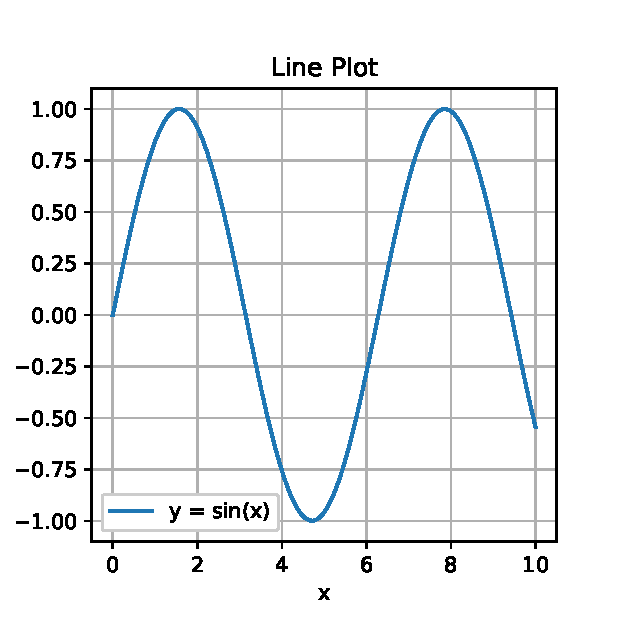
\includegraphics[width=0.99\linewidth]{mpl_plot_examples/line_plot.eps} %FILL IN THE PIC PATH HERE for plot
    \end{minipage}%
    \begin{minipage}{.25\textwidth}
      \centering
      \includegraphics[width=.99\linewidth]{mpl_plot_examples/scatter_plot.eps} %FILL IN THE PIC PATH HERE for scatter
    \end{minipage}
  \end{figure}

  \begin{figure}
    \centering
    \begin{minipage}{.25\textwidth}
      \centering
      \includegraphics[width=.99\linewidth]{mpl_plot_examples/bar_chart.eps} %FILL IN THE PIC PATH HERE for bar
    \end{minipage}%
    \begin{minipage}{.25\textwidth}
      \centering
      \includegraphics[width=.99\linewidth]{mpl_plot_examples/histogram.eps} %FILL IN THE PIC PATH HERE for hist
    \end{minipage}
    \begin{minipage}{.25\textwidth}
      \centering
      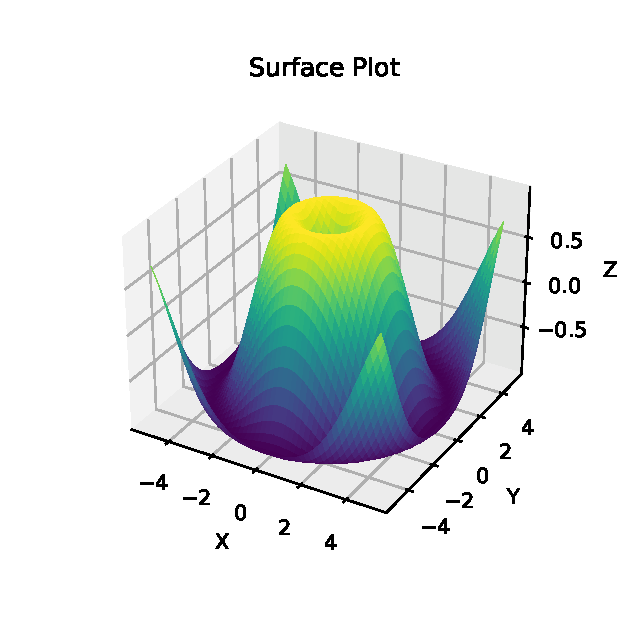
\includegraphics[width=.99\linewidth]{mpl_plot_examples/surface_plot.eps} %FILL IN THE PIC PATH HERE for surface
    \end{minipage}
  \end{figure}
\end{frame}



%%%% ALGORITHMS
\begin{frame}[fragile]
 \frametitle{Example algorithm}
 Compute the factorial of $N$: $N! = N\cdot(N-1)\cdot(N-2)\cdots 2\cdot 1$\\ \vskip1em
 How to deal with this? \vfill
 \begin{columns}[T]
  \column{0.3\textwidth}
  \begin{block}<2->{Naive approach}
      \begin{lstlisting}
Z = 1
Z = Z*2
Z = Z*3
Z = Z*4
... etc ...      
      \end{lstlisting}
  \end{block}
  \column{0.3\textwidth}
  \begin{block}<3->{For-loop}
      \begin{lstlisting}
Z = 1;
for i = range(N):
    Z = Z*i
end
      \end{lstlisting}
  \end{block}
  \column{0.3\textwidth}
\begin{block}<4>{While-loop}
      \begin{lstlisting}
Z = 1;
i = 1;
while i<=N:
    Z = Z*i
    i += 1
    \end{lstlisting}
  \end{block}
 \end{columns}
 \onslide<4>{
  Note: \lstinline$N$ must be set beforehand!\\ 
  Note: Pay attention to the relational operators!  }
\end{frame}

% INPUT AND OUTPUT
\begin{frame}[fragile]
  \frametitle{Input and Output in Python (1)}
  Many programs require some input (data) to function correctly. A combination of the following is common:
  \begin{itemize}[<+->]
    \item Input may be given in a parameters file (``hard-coded'')
    \item Input may be entered via the keyboard using the `input` function:
    \begin{lstlisting}[language=Python]
a = input('Please enter a number: ')
    \end{lstlisting}
    \item Input may be read from a file, for instance using Python's built-in open function or libraries like `numpy` for more complex data structures:
    \begin{lstlisting}[language=Python]
with open('myData.txt', 'r') as file:
    data = file.read()

import numpy as np
data = np.loadtxt("my_file.csv")
    \end{lstlisting}
    \item There are many other libraries and functions for more advanced input operations, such as json, xml, etc.
  \end{itemize}
 \end{frame}

 \begin{frame}[fragile]
  \frametitle{Input and Output in Python (2)}
  Output of results can be done in several ways, including:
  \begin{itemize}[<+->]
    \item Displaying results to the console - simply omitting a print statement will automatically show expression results in most Python IDEs.
    \item Using the `print` function to show results in the console:
    \begin{lstlisting}[language=Python]
 print("The result is:", result)
    \end{lstlisting}
    \item Saving data to a file can be done using various methods including writing to a file or using libraries like pandas for structured data:
    \begin{lstlisting}[language=Python]
with open('output.txt', 'w') as file:
     file.write(str(data))
 
data.save("data.npy")
    \end{lstlisting}
    \item More advanced output methods can utilize libraries such as NumPy, pandas, etc. to save data in various formats including JSON, Excel, etc.
  \end{itemize}
 \end{frame}
 


\begin{frame}[label=recursion,fragile]
 \frametitle{Advanced topic: Recursion}
 \begin{columns}
   \column{0.5\textwidth}
   \begin{itemize}
    \item<1-> In order to understand recursion, one must first understand recursion
    \item<2-> A recursive function includes a call to itself (a function within a function)
    \begin{itemize}
      \item<3-> This could lead to infinite calls;
      \item<3-> A base case is required so that recursion is stopped;
      \item<3-> Base case does not call itself, simply returns.
    \end{itemize}
 \end{itemize}
   \column{0.5\textwidth}
   \includegraphics<3>[width=0.7\columnwidth]{scoobydoo.jpg}
 \end{columns}
\end{frame}

% \againframe{recursion}

\begin{frame}[fragile]
 \frametitle{Recursion: example}
 \begin{lstlisting}[language=Python]
def mystery(a, b):
  if b == 1:
      # Base case
      return a
  else:
      # Recursive function call
      return a + mystery(a, b-1)
 \end{lstlisting}
\vskip1em \pause
\begin{itemize}
  \item What does this function do? \pause
  \item Can you spot the error? \pause
  \item How deep can you go? Which values of b don't work anymore?
\end{itemize}
\end{frame}

\begin{frame}[fragile]
 \frametitle{Recursion: exercise}
 Create a function computing the factorial of $N$, based on recursion. \pause
 \begin{lstlisting}[language=Python]
def fact_recursive(x):
    # Catch non-integer and negative cases
    if not isinstance(x, int) or x < 0:
        print("You should provide a positive integer number only")
        return None

    # Recursive case
    if x > 1:
        return x * fact_recursive(x - 1)

    # Base case
    else:
        return 1
 \end{lstlisting}
\end{frame}

\section{Conclusions}
\subsection*{Conclusions}
\againframe<2>{contents_prog1}
\begin{frame}[fragile]
  \frametitle{In conclusion...}
  \begin{itemize}
    \colorize<1> \item Python: A versatile development language. Easy to use libraries makes this language multi-purpose and easy to use.
    \colorize<2> \item Programming basics: variables, operators and functions, locality of variables, modules and recursive operations
  \end{itemize}
  \pause
    \begin{itemize}
    \colorize<3> \item For now: exercises on slide deck and Python modules
  \end{itemize}
\end{frame}

\section{Exercises}
\subsection*{Exercise 1}
\begin{frame}[fragile]
  \frametitle{Practice vectors and arrays}
  \begin{enumerate}
    \item Create a list \lstinline|x| with the elements:
    \begin{itemize}
      \item \lstinline|[2, 4, 6, 8, ..., 16]|
      \item \lstinline|[0, 0.5, 2/3, 3/4, ..., 99/100]|
    \end{itemize}
    \item Create a list \lstinline|x| with the elements: \(x_n = \frac{(-1)^n}{2n-1}\) for \(n=1,2,3,\ldots,200\). Find the sum of the first 50 elements \(x_1,\ldots,x_{50}\).
    \item Let \lstinline|x = list(range(20, 201, 10))|. Create a list \lstinline|y| of the same length as \lstinline|x| such that:
    \begin{itemize}
      \item \lstinline|y[i] = x[i] - 3|
      \item \lstinline|y[i] = x[i]| for every even index \(i\) and \lstinline|y[i] = x[i] + 11| for every odd index \(i\).
    \end{itemize}
    \item Let \lstinline|T = np.array([[3, 4, 6], [1, 8, 6], [-4, 3, 6], [5, 6, 6]])|. Perform the following operations on T:
    \begin{itemize}
      \item Retrieve a list consisting of the 2nd and 4th elements of the 3rd row.
      \item Find the minimum of the 3rd column.
      \item Find the maximum of the 2nd row.
      \item Compute the sum of the 2nd column
      \item Compute the mean of the row 1 and the mean of row 4
    \end{itemize}
  \end{enumerate}
 \end{frame}


 \begin{frame}[fragile]
  \frametitle{Practice plotting}
  \begin{enumerate}
    \item Plot the functions $f(x)=x,\ g(x)=x^3,\ h(x)=e^x$ and $z(x)=e^{x^2}$ over the interval $[0,4]$ on the normal scale and on the log-log scale. Use an appropriate sampling to get smooth curves. Describe your plots by using the functions: \lstinline$plt.xlabel$, \lstinline$plt.ylabel$, \lstinline$plt.title$ and \lstinline$plt.legend$.
    \vskip1em
    \item Make a plot of the functions: $f(x)=sin(1/x)$ and $g(x)=cos(1/x)$ over the interval $[0.01,0.1]$. How do you create \lstinline$x$ so that the plots look sufficiently smooth?
  \end{enumerate}
 \end{frame}

 \begin{frame}[fragile]
  \frametitle{Practice control flow and loops (1)}
  \begin{enumerate}
    \item Write a function that uses two logical input arguments with the following behaviour:
    \begin{align*}
       f(\text{true},\text{true}) \mapsto \text{false} \\
      f(\text{false},\text{true}) \mapsto \text{true} \\ 
      f(\text{true},\text{false}) \mapsto \text{true} \\
      f(\text{false},\text{false}) \mapsto \text{false} \\
    \end{align*}
    \item Write a function that computes the factorial of x:
    \[ f(x) = x! = 1 \times 2 \times 3 \times 4 \times \ldots \times x \]
    \begin{itemize}
      \item Using a loop-construction
      \item Using recursion
    \end{itemize}
  \end{enumerate}
 \end{frame}

 \begin{frame}[fragile]
  \frametitle{Practice control flow and loops (2)}
  \begin{enumerate}
    \item Write a function that computes the exponential function using the Taylor series
    \[  e^x = 1 + x + \frac{x^2}{2!} + \frac{x^3}{3!} + \ldots \]
    until the last term is smaller than $10^{-6}$.
    \item Use a script to compute the result of the following series:
    \[
      f_n = \sum_{n=1}^{\infty} \frac{1}{\pi^2 n^2}
    \]
    This should give you an indication of the fraction this series converges to.
    \begin{itemize}
      \item Now plot in two vertically aligned subplots i) The result as a function of $n$, and ii) the difference with the earlier mentioned fraction as a function of n. For the latter, consider carefully the axis scale!
      % \item Use \lstinline$tic$ and \lstinline$toc$ to compare the computing times with $\pi^2$ inside vs outside the loop.
    \end{itemize}
  \end{enumerate}
 \end{frame}

 \begin{frame}[fragile]
  \frametitle{Practice logical indexing}
  \begin{enumerate}
    \item Let \lstinline$x = np.linspace(-4,4,1000)$, $y_1 = 3x^2 - 4x - 6$ and $y_2 = 1.5x - 1$. Use logical indexing to determine function $y_3 = \mathrm{max}(\mathrm{max}(y_1,y_2),0)$. Plot the function.
    \item Consider these data concerning the age (in years), length (in cm) and weight (in kg) of twelve adult men: \lstinline$A = [41 25 33 29 64 34 47 38 49 32 26 26]; H = [165 186 177 190 156 174 164 205 184 190 165 171]; W = [75 90 97 60 74 65 101 85 91 75 87 70];$.
    \begin{itemize}
      \item Calculate the average of all vectors (age, weight and length).
      \item Combine the command \lstinline$length$ with logical indexing to determine how many men in the group are taller than 182 cm.
      \item What is the average age of men with a body-mass index ($B \equiv \frac{W}{L^2}$ with $W$ in kg and $L$ in m) larger than 25? And for men with a $B<25$?
      \item How many men are older than the average and at the same time have a BMI below 25?
    \end{itemize}
  \end{enumerate}
 \end{frame}

\begin{frame}[fragile]
  \frametitle{Practice algorithm: Fourier series for heat equation}
  The unsteady 1D heat equation in 1D in a slab of material is given as:
  \[
     \frac{\partial T}{\partial t} = k\frac{\partial^2 T}{\partial x^2}
  \]
 We can express the temperature profile $T(x,t)$ in the slab using a Fourier sine series. For an initial profile T(x,0) = 20 and fixed boundary values T(0,t) = T(L,t) = 0, the solution is given as:
  \[
     T(x,t) = \sum_{n=1}^{n=\infty}\frac{40(1-(-1)^n)}{n\pi}  \sin\left(\frac{n\pi x}{L}\right) \exp\left(-kt\frac{n \pi}{L}^2\right)
  \]
  \begin{itemize}
      \item Create a script to solve this equation using loops and/or conditional statements
  \end{itemize}
 \end{frame}
 
%  \begin{frame}[fragile]
%   \frametitle{Fourier series for heat equation (1)}
%   A simple construct with a double loop.
%    \begin{lstlisting}
%  L = 2;
%  k = 0.004;
%  t = 3;
%  x = 0:0.1:L;
%  s = 0;
 
%  for n = 1:50
%      for i = 1:length(x)
%          pt(i) = 40*(1-(-1)^n)/(n*pi) * sin(n*pi*x(i)/L) * exp(-k*t*(n*pi/L)^2);
%      end
%      s = s + pt;
%  end
 
%  plot(x,s)
%    \end{lstlisting}
%  \end{frame}
 
%  \begin{frame}[fragile]
%   \frametitle{Fourier series for heat equation (2-1)}
%  We can also solve the equation for the entire x-range in 1 go. \lstinline$part$ and $s$ are both vectors. This is more efficient.
%    \begin{lstlisting}
%  L =  2;
%  x = linspace(0,L,101);
%  k = 0.004;
%  t = 3;
 
%  s = 0;
%  for n = 1:50
%      part = 40*(1-(-1)^n)/(n*pi) * sin(n*pi*x/L) * exp(-k*t*(n*pi/L)^2);
%      s = s + part;
%  end
 
%  plot(x,s)
%    \end{lstlisting}
%  \end{frame}
 
%  \begin{frame}[fragile]
%   \frametitle{Fourier series for heat equation (2-2)}
%  We can break the for-loop when the calculations are precise enough using an if-statement and a break-command.
%    \begin{lstlisting}
%  L = 2;
%  x = linspace(0,L,101);
%  k = 0.004;
%  t = 3;
 
%  s = 0;
%  for n = 1:2:50
%      part = 40*(1-(-1)^n)/(n*pi) * sin(n*pi*x/L) * exp(-k*t*(n*pi/L)^2);
%      s = s + part;
%      if (max(abs(part)) < 1e-6)
%          n
%          break
%      end
%  end
 
%  plot(x,s)
%    \end{lstlisting}
%  \end{frame}
 
%  \begin{frame}[fragile]
%   \frametitle{Fourier series for heat equation (3-1)}
%  We can run a while-loop for indeterminate iterations to ensure a certain precision while keeping computational demands to a minimum:
%    \begin{lstlisting}
%  L =  2;
%  x = linspace(0,2,101);
%  k = 0.004;
%  t = 3;
 
%  s = 0;
%  n = 1;
%  part = 1;
%  while (max(abs(part))>1e-6)
%      part = 40*(1-(-1)^n)/(n*pi) * sin(n*pi*x/L) * exp(-k*t*(n*pi/L)^2)
%      s = s + part;
%      n = n + 2;
%  end
 
%  n
%  plot(x,s)
%    \end{lstlisting}
%  \end{frame}
 
%  \begin{frame}[fragile]
%   \frametitle{Fourier series for heat equation (3-2)}
%  The \lstinline$drawnow$ command makes sure a plot is drawn before subsequent commands are executed. This gives us insight in the iteration process:
%    \begin{lstlisting}
%  L =  2;
%  x = linspace(0,2,101);
%  k = 0.004;
%  t = 3;
 
%  s = 0;
%  n = 1;
%  part = 1;
%  while (max(abs(part))>1e-6)
%      part = 40*(1-(-1)^n)/(n*pi) * sin(n*pi*x/L) * exp(-k*t*(n*pi/L)^2)
%      s = s + part;
%      n = n + 2;
%      plot(x,s)
%      pause(0.4)
%      drawnow
%  end
 
%  n
%    \end{lstlisting}
%  \end{frame}

%  \begin{frame}[fragile]
%   \frametitle{Fourier series for heat equation (as a function)}
%  A rudimentary function (i.e. no comments or checks) to get the heat equation profile for a given length, heat diffusivity and time:
%    \begin{lstlisting}
%  function [s,x] = fourier_series_heat_eqn(L,k,t)
%  x = linspace(0,L,101);
 
%  s = 0;
%  n = 1;
%  part = 1;
%  while (max(abs(part))>1e-6)
%      part = 40*(1-(-1)^n)/(n*pi) * sin(n*pi*x/L) * exp(-k*t*(n*pi/L)^2);
%      s = s + part;
%      n = n + 2;
%  end
%    \end{lstlisting}
   
%  Calling the function from a different script multiple times to plot a transient profile:
%  \begin{lstlisting}
%  for t = 0.01:0.01:30
%      [solution,xvec] = fourier_series_heat_eqn(2,0.004,t);
%      plot(xvec,solution)
%      xlabel('Position [m]');
%      ylabel('Temperature [^\circC]');
%      drawnow
%  end
%  \end{lstlisting}
%  \end{frame}

% \end{document}


% References
% http://ocw.mit.edu/courses/electrical-engineering-and-computer-science/6-00sc-introduction-to-computer-science-and-programming-spring-2011/unit-1/lecture-1-introduction-to-6.00/
% http://www.greenteapress.com/thinkpython/html/thinkpython002.html
% https://www.youtube.com/channel/UCLMQ21H2ad95faYG3yGCwYA
%http://stackoverflow.com/questions/4227145/in-Python-are-variables-really-double-precision-by-default
%http://www.exploringbinary.com/why-0-point-1-does-not-exist-in-floating-point/

